% Working draft. OPEN DECISIONS (owner): venue, page limit, template. Until decided: generic
% article class, 11pt, ~8-10 pages. Tables and figures are generated from the result artifacts by
%   python -m research.paper.make_paper_assets
% Every number in the text is taken from research/artifacts/*.json (see research/REPRODUCE.md).
\documentclass[11pt]{article}
\usepackage[margin=1in]{geometry}
\usepackage{iftex}
\ifPDFTeX
  \usepackage[T1]{fontenc}
  \usepackage[utf8]{inputenc}
\fi
\usepackage{lmodern}
\usepackage[section]{placeins}   % floats stay inside their section
\usepackage{amsmath}
\usepackage{booktabs}
\usepackage{graphicx}
\usepackage{xcolor}
\usepackage[round]{natbib}
\usepackage[hidelinks]{hyperref}

\newcommand{\affectedrule}{precision 40.6\%, recall 90.0\%, F1 0.56; AUC of the expected move 0.56}
        % generated numbers used inside captions
\newcommand{\tbd}[1]{\textcolor{red}{[TBD: #1]}}
\newcommand{\bps}{\,bps}   % write \bps{} before a space

\title{From Headline to Currency Reaction: Predicting Affected Pairs, Direction, Magnitude and
Confidence of FX Moves from News, for Ranking Arbitrage Opportunities}
\author{\tbd{authors}}
\date{\tbd{date}}

\begin{document}
\maketitle

\begin{abstract}
Cross-venue foreign-exchange (FX) arbitrage systems detect price discrepancies but cannot tell
which of them news makes dangerous. We build and evaluate a semantic layer that, for each
incoming article, states which currency pairs are affected, in which direction, by how much and
with what calibrated confidence. For scheduled macroeconomic releases, a structured pipeline
grounded in 1,385 high-impact releases (2018--2025, four major pairs, one-minute bars)
identifies the direction of the 15-minute release reaction 68.4\% of the time with a
theory-signed surprise rule, with calibrated confidence (expected calibration error 0.04) and
conformal intervals for the move size. Under a pre-registered walk-forward design, a learned
per-cell response model does \emph{not} beat the theory rule (63.5\%), and from the moment a news
article typically arrives, 15 minutes after the release, no direction remains to predict
(48.8\%, $p=0.27$): the reaction is complete within a minute and then persists. We document three
silent errors in widely used free data (calendar timestamps, price-file daylight saving and news
API truncation), each of which changes a conclusion, and disclose a contamination of the live
pipeline by synthetic demo headlines found during the study. \tbd{unscheduled-news results
(H1, H5, H6), prospective live test, ranking value.}
\end{abstract}

\section{Introduction}

A cross-venue arbitrage detector flags moments when one venue's bid exceeds another's ask. Once
both legs fill, such a position is close to market-neutral; what remains is execution risk ---
legging exposure while the second leg is pending, and stale quotes around news. A semantic layer
is useful to such a system only if it answers, for each article and each pair: is this pair
affected, which way does it move, by how much, and how sure is the answer? ``How sure'' has to be
a probability that means what it says, because it is used as a weight.

We make four contributions.
(i) A pre-registered evaluation of an article-to-reaction pipeline for scheduled releases, which
separates the reaction measured from the release from what is still predictable when an article
arrives (Section~\ref{sec:results}).
(ii) Evidence that a theory-signed surprise rule beats a learned response model out of sample,
and that confidence can be calibrated but carries little resolution at 15 minutes.
(iii) Three silent errors in free FX and news data, each shown to change a result
(Section~\ref{sec:data}).
(iv) A deployed microservice and a prospective test of it, including the disclosure of a data
contamination that a less careful audit would have missed (Section~\ref{sec:live}).

\section{Related work}
High-frequency FX responses to macroeconomic announcements are documented by
\citet{abdv2003}, \citet{faust2007} and \citet{evanslyons2008}: surprises move exchange rates
within minutes, with signs that follow economic priors. Our scheduled-release study replicates
this on corrected data and turns it into an article-level predictor. \citet{tetlock2011} shows
that markets react less to stale news, which motivates the semantic-novelty hypothesis of our
unscheduled-news arm; \citet{bbd2016} build news-based indices of the kind our currency-level
sentiment factor follows. Sentiment baselines use FinBERT \citep{araci2019}; novelty uses
sentence embeddings \citep{reimers2019}; unscheduled news comes from GDELT \citep{leetaru2013}.
Inference follows cluster-robust practice \citep{cameronmiller2015} with false-discovery control
\citep{bh1995}; intervals are split-conformal \citep{lei2018}; calibration is measured as in
\citet{guo2017}. The study is pre-registered \citep{nosek2018}.

\section{Data, and three silent errors}\label{sec:data}

\paragraph{Sources.} An economic-calendar dump in ForexFactory format (34,333 events,
2018-01 to 2025-04; 2,778 high-impact releases with an exact time and a standardized surprise);
HistData one-minute bid bars for EUR/USD, GBP/USD, USD/JPY and USD/CHF (2018--2025); the GDELT
DOC 2.0 API for English news. Surprises are standardized per (currency, indicator) by a $\sigma$
estimated outside 2020-03-01..2021-06-30 and winsorized at $\pm5\sigma$.

\paragraph{Error 1: calendar timestamps.} Missing times are stored as local midnight (about 30\%
of rows, including all 88 payrolls releases of 2018--2025), and the dump's UTC offsets still
apply a daylight-saving rule abolished in 2022. Our pre-registered positive control failed twice
on these clocks; on corrected clocks the original specification passes all three criteria
(payrolls 5-minute EUR/USD $\beta=-8.99$\bps/$\sigma$, $p=0.010$; pooled $+6.51$, $p<10^{-10}$;
placebo $p=0.33$), reported as post hoc. Table~\ref{tab:pc} gives the corrected pooled responses.

\paragraph{Error 2: daylight saving in price files.} The one-minute files described as fixed
Eastern Standard Time are New York wall-clock time with daylight saving. The symptom was a
reaction ``jump'' exactly 60 minutes after every summer release; under the documented clock the
summer one-minute reaction is $+0.5$\bps, after the fix $+8.5$\bps.

\paragraph{Error 3: news API truncation.} A 24-hour GDELT DOC request with newest-first sorting
and the 250-record cap returns only the minutes before midnight UTC (Figure~\ref{fig:gdelt}). The
daily sample is therefore not a sample of the trading day; it is withdrawn and replaced by a
time-stratified sample of one-hour slices (Section~\ref{sec:prereg}).

\begin{table}[t]\centering\small
\caption{Positive control on corrected clocks: pooled sign-oriented response to a one-$\sigma$ US
surprise at one minute (standard errors clustered by release).}\label{tab:pc}
\begin{tabular}{lrrrrr}
\toprule
Pair & $\beta$ (bps/$\sigma$), 1 min & $p$ & $R^2$ & $n$ & Release clusters \\
\midrule
EUR/USD & 4.43 & $<$0.001 & 0.12 & 1374 & 771 \\
GBP/USD & 4.20 & $<$0.001 & 0.11 & 1374 & 778 \\
USD/JPY & 5.34 & $<$0.001 & 0.12 & 1384 & 779 \\
USD/CHF & 4.29 & $<$0.001 & 0.11 & 1377 & 778 \\
\bottomrule
\end{tabular}

\end{table}

\begin{figure}[t]\centering
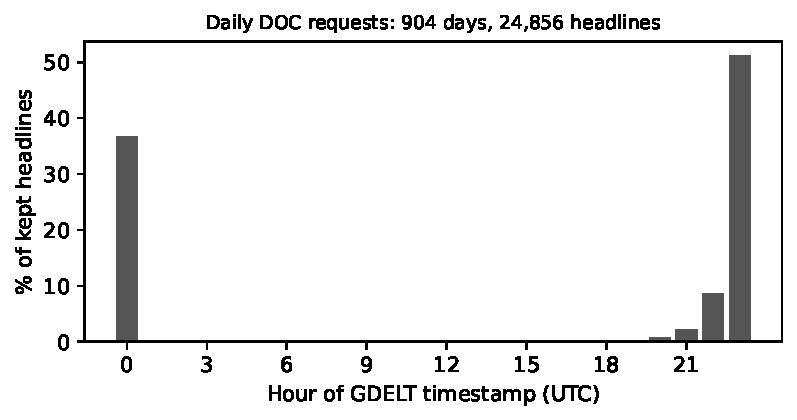
\includegraphics[width=0.8\linewidth]{figures/gdelt_daily_defect.pdf}
\caption{Time of day of headlines kept by daily GDELT DOC requests: 88\% are stamped between
23:00 and 01:00 UTC.}\label{fig:gdelt}
\end{figure}

\section{Pre-registration and design}\label{sec:prereg}
Hypotheses, metrics, baselines and stop rules were fixed in a dated, append-only tracker before
results; departures are numbered deviations with reasons, all made before the affected results
existed (cutoff moves after laptop downtime; the GDELT re-collection after the truncation was
found by a timestamp-only check). \tbd{appendix table of deviations and clarifications C1--C32.}

\paragraph{Unit and targets.} Each high-impact, exact-time release with $z\neq0$ in USD, EUR,
GBP, JPY or CHF (1,385 releases) $\times$ each of the four majors. Release-time returns
$r(0,h)$ for $h\in\{1,5,15,30,60,120\}$ minutes (primary 15); arrival-time returns
$r(15,15+h)$ for $h\in\{15,45,105\}$ (primary 15--60), because an article reporting a release
arrives after it. Returns are log returns in bps between the first bars at or after the window
ends (bars stamped at close; entry lag $\le2$, exit lag $\le5$ minutes, fail closed).

\paragraph{Model.} Direction $\hat s=\operatorname{sign}(\hat\beta z)$ with $\hat\beta$ estimated
through the origin per (release currency, category, pair); expected move
$|r| = a + b|z| + c\,v$ with $v$ the same-clock mean absolute return over the previous 20
weekdays; confidence $P(\hat s\text{ correct}\mid|z|)$ by logistic regression; split-conformal
intervals for $|r|$. Expanding monthly walk-forward with 12 training-only months gives 76 test
months (2019-01 to 2025-04); inference is clustered by release moment (about 900 clusters).

\section{Results: scheduled releases}\label{sec:results}

\paragraph{Direction (RQ2).} Table~\ref{tab:dir}. The release reaction is predictable --- 75.2\%
at one minute and 68.4\% at 15 minutes for the theory rule $\operatorname{sign}(z)\times$(the
indicator's economic sign) --- but the learned model is \emph{worse} than that rule at every
horizon: the learned $\hat\beta$ agrees with the theory sign on 82\% of rows, and the
disagreements are noise from small cells. Accuracy rises with $|z|$. From article arrival
there is no direction left: 48.8\% for the primary 15--60 minute window ($p=0.27$), and the mean
move in the predicted direction is 7--8\bps{} from 1 to 120 minutes after the release but
indistinguishable from zero after arrival (Figure~\ref{fig:profile}).

\begin{table}[t]\centering\scriptsize
\caption{Direction accuracy (\%) out of sample. $^\dagger$primary. Rows: release $\times$ own
pair; moments: release clusters.}\label{tab:dir}
\resizebox{\linewidth}{!}{\begin{tabular}{lrrrrrrr}
\toprule
Window (min after release) & Model acc. [95\% CI] & AUC & Theory rule acc. [95\% CI] & Majority & $p$ (model vs.\ 50\%) & Rows & Moments \\
\midrule
release, 0--1 & 68.2 [65.2, 71.1] & 0.75 & 75.2 [72.5, 77.7] & 51.5 & $<$0.001 & 3,667 & 897 \\
release, 0--5 & 64.6 [61.9, 67.3] & 0.71 & 71.8 [69.2, 74.4] & 52.4 & $<$0.001 & 3,680 & 899 \\
release, 0--15$^\dagger$ & 63.5 [60.2, 66.5] & 0.67 & 68.4 [65.4, 71.3] & 51.5 & $<$0.001 & 3,687 & 900 \\
release, 0--30 & 62.0 [59.1, 65.1] & 0.66 & 66.4 [63.5, 69.3] & 51.2 & $<$0.001 & 3,676 & 896 \\
release, 0--60 & 60.4 [57.3, 63.5] & 0.62 & 64.4 [61.5, 67.2] & 51.8 & $<$0.001 & 3,568 & 860 \\
release, 0--120 & 57.7 [55.3, 60.2] & 0.60 & 61.0 [58.2, 63.8] & 52.2 & $<$0.001 & 3,656 & 895 \\
\midrule
arrival, 15--30 & 47.9 [45.6, 50.4] & 0.47 & 50.5 [47.7, 53.4] & 51.5 & 0.082 & 3,683 & 901 \\
arrival, 15--60$^\dagger$ & 48.8 [46.6, 51.0] & 0.49 & 51.0 [48.0, 53.7] & 50.5 & 0.265 & 3,555 & 862 \\
arrival, 15--120 & 50.2 [48.0, 52.2] & 0.49 & 50.1 [47.4, 53.1] & 49.7 & 0.852 & 3,635 & 894 \\
\bottomrule
\end{tabular}
}
\end{table}

\begin{figure}[t]\centering
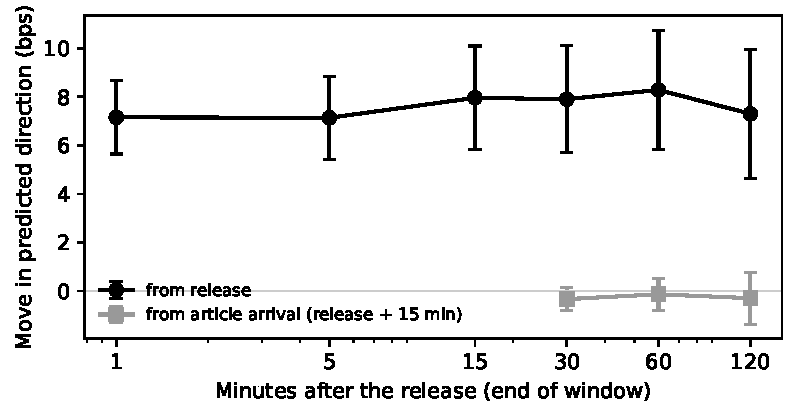
\includegraphics[width=0.8\linewidth]{figures/horizon_profile.pdf}
\caption{Mean move in the predicted direction with 95\% intervals (release-moment clustered).
The reaction is complete within a minute and persists; nothing remains after arrival.}\label{fig:profile}
\end{figure}

\paragraph{Magnitude (RQ3).} Table~\ref{tab:mag}. The model ranks moves better than the
training-mean baselines (Spearman 0.29 vs 0.19 at 15 minutes) but its mean absolute error is not
lower than any baseline's, and after arrival the same-clock volatility baseline beats it.

\begin{table}[t]\centering\scriptsize
\caption{Magnitude: MAE (bps) / Spearman; in parentheses the model-minus-baseline absolute error
and its clustered $p$-value.}\label{tab:mag}
\resizebox{\linewidth}{!}{\begin{tabular}{lrllll}
\toprule
Window & Mean $|r|$ & Model & Pair mean & Cell mean & Same-clock $v$ \\
\midrule
release, 0--15$^\dagger$ & 16.2 & 12.01 / 0.29 & 11.54 / 0.19 (+0.47, $p=0.150$) & 11.59 / 0.24 (+0.42, $p=0.090$) & 11.85 / 0.29 (+0.16, $p=0.455$) \\
release, 0--60 & 20.4 & 14.32 / 0.23 & 13.98 / 0.15 (+0.34, $p=0.317$) & 14.04 / 0.20 (+0.28, $p=0.271$) & 14.39 / 0.23 (-0.07, $p=0.719$) \\
arrival, 15--60$^\dagger$ & 11.2 & 7.40 / 0.16 & 7.27 / 0.07 (+0.12, $p=0.172$) & 7.43 / 0.08 (-0.04, $p=0.614$) & 7.11 / 0.22 (+0.29, $p<0.001$) \\
\bottomrule
\end{tabular}
}
\end{table}

\paragraph{Confidence (RQ4).} Table~\ref{tab:conf}, Figure~\ref{fig:rel}. Confidence is
calibrated (ECE 0.04 at 15 minutes) but has little resolution there (Brier 0.234 against 0.232
for a constant rate); at one minute it does better than a constant. Conformal intervals cover
77\% and 87\% at nominal 80\% and 90\%.

\begin{table}[t]\centering\scriptsize
\caption{Calibration of $P(\text{direction correct})$ and conformal coverage of the move size.}\label{tab:conf}
\resizebox{\linewidth}{!}{\begin{tabular}{lrrrrrrrr}
\toprule
Window & ECE & Brier & Brier (const.) & Mean $p$ (\%) & Hit rate (\%) & Cov.\ 80\% & Cov.\ 90\% & 90\% width (bps) \\
\midrule
release, 0--1 & 0.042 & 0.207 & 0.217 & 72.1 & 68.2 & 76.8 & 87.0 & 32.6 \\
release, 0--15$^\dagger$ & 0.041 & 0.234 & 0.232 & 65.1 & 63.5 & 76.5 & 86.9 & 41.2 \\
release, 0--60 & 0.046 & 0.242 & 0.239 & 58.7 & 60.4 & 76.4 & 86.9 & 47.0 \\
arrival, 15--60$^\dagger$ & 0.056 & 0.259 & 0.250 & 53.2 & 48.8 & 78.5 & 89.1 & 25.6 \\
\bottomrule
\end{tabular}
}
\end{table}

\begin{figure}[t]\centering
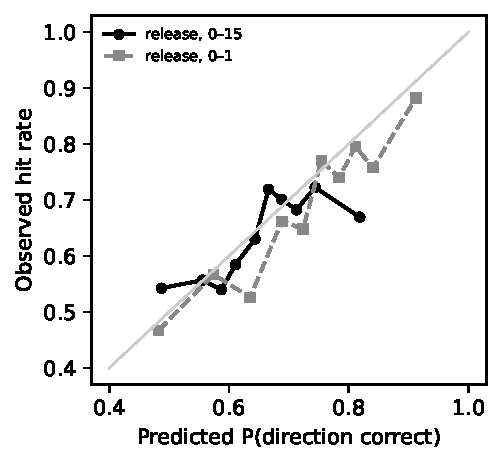
\includegraphics[width=0.45\linewidth]{figures/reliability.pdf}
\caption{Reliability of the confidence output (equal-mass bins).}\label{fig:rel}
\end{figure}

\paragraph{Affected pairs (RQ1).} Table~\ref{tab:aff}. The currency rule (a pair is affected if it
contains the release currency) recalls 90\% of abnormal moves with 41\% precision; a euro-area
release moves GBP/USD and USD/JPY abnormally about 22\% of the time.

\begin{table}[t]\centering\small
\caption{Share (\%) of release $\times$ pair rows with an abnormal 15-minute move ($|r|>2v$). Rows with
few releases (JPY, CHF) are anecdotal. Currency rule (affected if the pair contains the release
currency): \affectedrule.}\label{tab:aff}
\begin{tabular}{lrrrr}
\toprule
Release currency & EUR/USD & GBP/USD & USD/JPY & USD/CHF \\
\midrule
CHF & 29 & 33 & 14 & 76 \\
EUR & 52 & 22 & 23 & 17 \\
GBP & 17 & 40 & 17 & 16 \\
JPY & 100 & 100 & -- & -- \\
USD & 40 & 37 & 43 & 40 \\
\midrule
\multicolumn{5}{l}{Currency rule: precision 40.6\%, recall 90.0\%, F1 0.56; AUC of expected move 0.56} \\
\bottomrule
\end{tabular}

\end{table}

\paragraph{Categories.} Release categories differ in size (inflation $>$ employment $>$ growth),
all within a minute and persistent (Table~\ref{tab:h2}).

\begin{table}[t]\centering\small
\caption{Sign-oriented cumulative response by category (bps), US releases, four majors pooled;
$^{*}$survives Benjamini--Hochberg at $q\le0.05$.}\label{tab:h2}
\begin{tabular}{lrrrrr}
\toprule
Category & 1 min & 15 min & 60 min & 120 min & Release dates \\
\midrule
inflation & 17.3$^{*}$ & 19.1$^{*}$ & 20.9$^{*}$ & 20.6$^{*}$ & 132 \\
employment & 7.6$^{*}$ & 7.7$^{*}$ & 8.4$^{*}$ & 8.3$^{*}$ & 256 \\
growth & 5.4$^{*}$ & 5.6$^{*}$ & 5.9$^{*}$ & 4.9$^{*}$ & 336 \\
\bottomrule
\end{tabular}

\end{table}

\section{Unscheduled news (H1, H5, H6)}
\tbd{results after the 2026-11-10 freeze of the time-stratified GDELT slice sample.}

\section{Live system and prospective test}\label{sec:live}
The detector (Arbex backend) passes each opportunity to the ranking channels; the semantic
microservice matches release headlines to the live calendar and returns per-pair direction,
calibrated probability, expected move and whether the move is already priced in.
\paragraph{Contamination disclosure.} During the study we found that the live feed filled quiet
periods with synthetic demo headlines: 92\% of logged predictions before 2026-11-02, and 26\%
of the USD/INR training rows of the earlier text model. They are excluded from every analysis,
the text-model baseline is retrained without them, and analyses of the live ranking inputs are
reported both for the pre-registered window and for the clean window.
\paragraph{Venue caveat.} The recorded ``opportunities'' compare Kraken with TrueFX, an indicative
aggregated feed; they are price discrepancies, not executable arbitrage.
\tbd{prospective test; arrival latency; real-headline extraction (RQ2-E2E); ranking value (RQ5).}

\section{Discussion}
For a ranker, the direction a release article reports describes a move that has already
happened. Its value lies in identifying which venue's quote is stale and in pricing the
release window as execution risk, not in forecasting what follows. Calibration matters more
than raw accuracy for a weighting factor. The data errors we found were silent and biased results
toward a null; checking clocks against a known effect before testing new hypotheses was what
exposed them.

\section{Limitations}
No free intraday data exist for USD/INR; JPY and CHF releases are few (3 and 30). News is
headlines only, timestamped by GDELT to 15 minutes, and sampled by slices. The H2 and
positive-control analyses used the same 2018--2025 releases, so walk-forward testing is the
out-of-sample evidence for RQ1--RQ4. The sample cutoff moved twice and the news sample was
re-collected once, each before the affected results existed.

\bibliographystyle{plainnat}
\bibliography{references}
\end{document}
